\chapter{Historic Perspective on the Structure of Matter and Spin}
\section{The Phenomena of Spin}

Spin is a fundamental quantity possessed by all elementary particles. We use
the word 'spin' to describe the property, because particles which possess spin,
behave as though they have some kind of intrinsic, hidden rotation, as if they
were 'spinning'. The dimension of spin, therefore is angular momentum. What is
somewhat bizarre about spin, is that we do not observe anything physically
spinning - although there are some phenomena (such as orbital angular momenta)
which can be naively thought of as a 'spinning system' (but this description
escapes classical analogy, due to its quantum, probabilistic nature). The role
of Spin in Physics is of foundational importance, and yet, we have not
successfully produced a model which can accurately predict the spin of hadrons.

The presence of spin in relativistic particles creates the phenomena of
chirality, which has huge implications for how elementary particles can generate
structure in matter itself~\cite{Brodsky1988}. In the case of the weak
interaction, the presence of spin, which creates Chiral spinors breaks the
left-right symmetry of weak coupling in matter (a fact which will be exploited
in this thesis to probe the spin of the proton sea).

The phenomena of spin also changes the rules for how ensembles of particles may
exist in a potential. Particles with spin are fermions, and because these
particles must obey Fermi-statistics, we can observe structure in matter in the
universe. Without spin, the world as we know would collapse on itself, making
any kind of extended non-exotic structures which currently exist by virtue of
the Pauli exclusion principal, impossible.

\clearpage
\section{A Brief History of Relevant Physics}

The study of Spin is really just an outgrowth of the general study of matter.
Our models for matter, and the underlying structure of matter (in the modern
sense), represents over a hundred years of experimental and theoretical efforts,
and thousands of years of contemplating what makes up the universe.

Although indulgent on my part, I find it interesting, and humbling, to try and
map out the path that humanity and science has trodden on its way to
understanding the building blocks of the universe. To find the first time that
humanity had murmurings that suggested our visible world is built from
invisible, fundamental building blocks, we must travel back, nearly 2,500 years
into the past.

Rather than provide a complete mathematical background to my measurement from a
historic perspective, I will instead focus on the experimental historic
narrative surrounding our quest to understand the structure of matter. After, I
will present mathematical formalism relevant to this measurement directly - if
the reader desires an exhaustive mathematical context, I invite them to read the
classic tomes on Field Theory by Weinberg and reference the numerous theses
written by my colleagues in theoretical physics and phenomenology.

\section{Ancient Foundations}
Sometime around 490 - 370 BCE lived two philosophers, Empedocles
(Fig~\ref{fig:empedocles}), and Democrtius (Fig~\ref{fig:democritus}). Both men
lived approximately at the same time, and made huge philosophical leaps in
attempting to understand the nature of the visible world.

\begin{figure}[ht]
	\centering
	\begin{subfigure}{.5\textwidth}
		\centering
		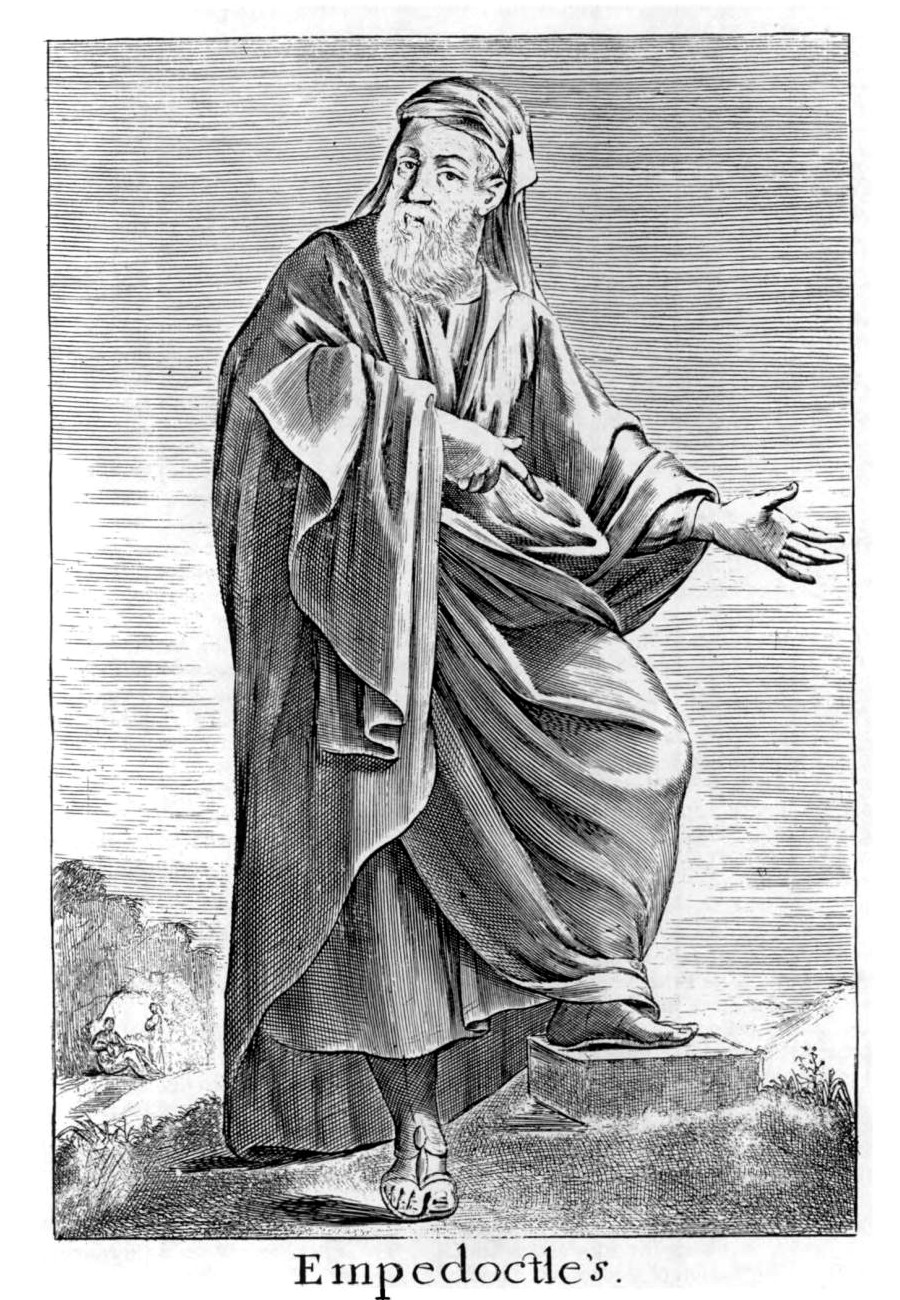
\includegraphics[width=0.4\linewidth]{./figures/empedocles.jpg}
		\caption{Empedocles \cite{Stanley1655}}
		\label{fig:empedocles}
	\end{subfigure}%
	\begin{subfigure}{0.5\textwidth}
		\centering
		
\includegraphics[width=0.4\linewidth]{./figures/democritus.jpg}
		\caption{Democritus \cite{Brugghen1628}}
		\label{fig:democritus}
	\end{subfigure}
  \caption{ 
    Two Greek philosophers, who made important philosophical
    contributions our understanding of matter. Empedocles (left), postulated the
    precursor to the elemental theory of matter\cite{Long1949} and Democritus
    (right), postulated the precursor to the atomic theory of matter.  
  }
	\label{fig:atomists}
\end{figure}

Democritus was part of a movement of thought which was first to make the
intellectual jump that perhaps matter was not a continuum, but instead, composed
of 'atomon', small, indivisible particles which when configured together, created
all that is observable~\cite{Baldes1978}. Empedocles was making equally important
philosophical strides - in a manner complimentary to Democritus' opinion that
matter must be made of atomon, Empedocles argued that matter is composed of
elemental primitives~\cite{Long1949}.

Although Empedocles' 'periodic table' was only composed of Earth, Water, Fire,
and Air, the idea that some unseen transmutation of elemental forces might
generate observables in nature with quite different (but perhaps reminiscent)
properties then the 'pure substances' was an important step forward.
Proto-scientists were beginning to generate models which derived our complicated
observations, from simpler forms.

It took centuries of cultivation, leading up to the Scientific Revolution, for
the next great steps to occur, for science. Thankfully, the luminaries of the
Islamic Golden Age kept the fires of inquiry burning~\cite{Alexakos2005}.

\clearpage
\section{The Scientific Revolution}

Thanks to the mathematical foundations laid out, build, and maintained by the
minds of the Islamic Golden Age, Europe was well poised to reignite the flames
of scientific inquiry, during the post Renaissance Scientific
Revolution~\cite{Alexakos2005}.

This period of growth in science was unprecedented during the Scientific
Revolution, thanks to the seeds of empiricism germinated during the Islamic
Golden Age, fertilized by the Italian Renaissance, and helped to flourish
through British Empiricism~\cite{Cowley1968}.

\begin{figure}[ht]
	\centering
	\begin{subfigure}{.5\textwidth}
		\centering
		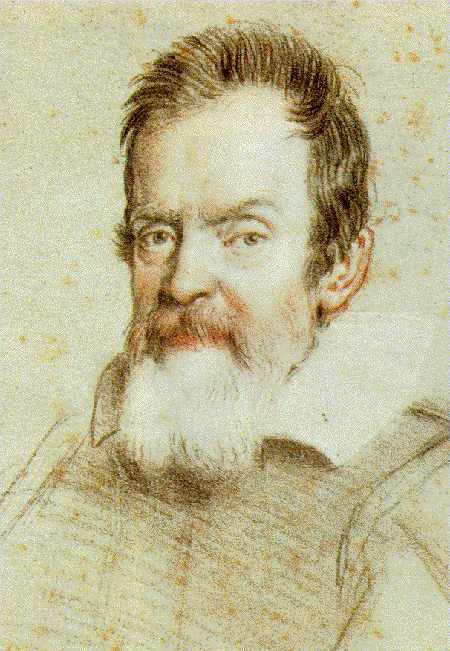
\includegraphics[width=0.4\linewidth]{./figures/galileo.jpg}
		\caption{Galileo \cite{Leoni1624}}
		\label{fig:galileo}
	\end{subfigure}%
	\begin{subfigure}{0.5\textwidth}
		\centering
		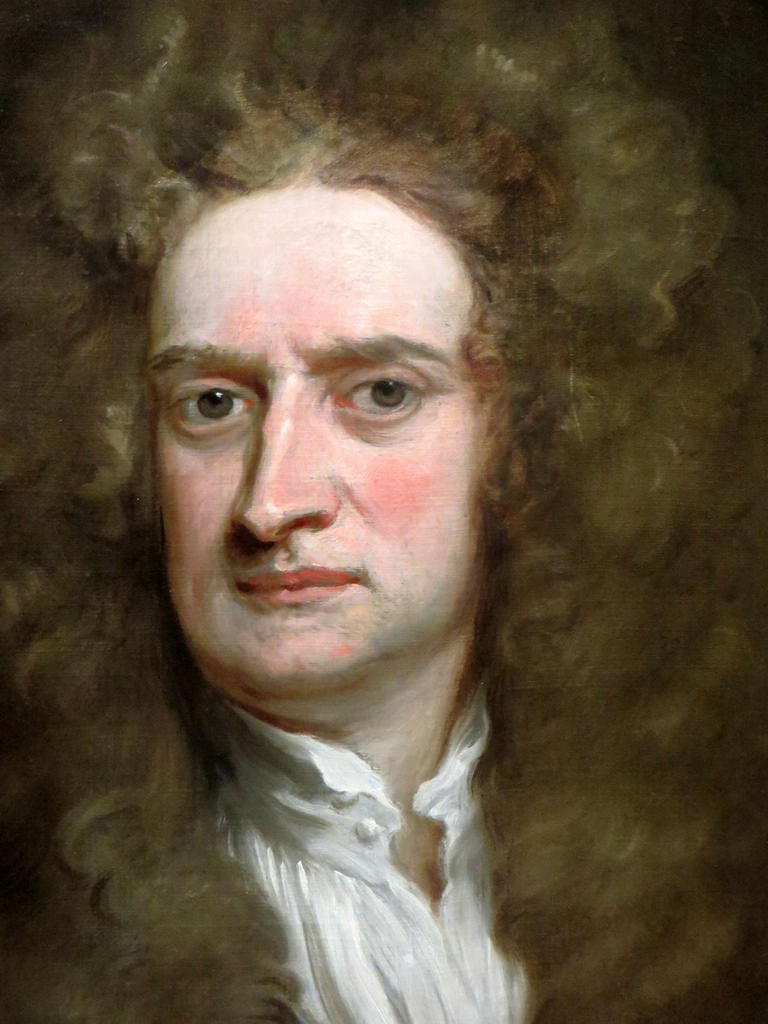
\includegraphics[width=0.4\linewidth]{./figures/newton.jpg}
		\caption{Newton}
		\label{fig:newton}
	\end{subfigure}
	\caption{ 
		Giants in the age of Empiricism, Newton (left) and
		Galileo (right) both made foundational contributions to Physics.
		Galileo lived in Italy, born in 1564 and dying in 1642. Newton lived in
		England from 1642 until his death in 1727
	}
	\label{fig:newtongalileo}
\end{figure}

\subsection{Galileo Galilei}
While Galileo is best known for his work in Observational Astronomy, his
importance to science extends beyond this. During his years in exile for his
controversial views of the heliocentric universe, he produced some of his most
important scientific work in kinematics~\cite{Hall1965}. What made this work
remarkable is the care that Galileo took in merging careful mathematical
modeling with well designed experimentation. This methodical approach to inquiry
laid the foundation for others to slowly begin to pull back the curtains
obscuring physical law.

Galileo's formalization of the scientific method inexorably set science on a
course to delving deep into the nature of matter, and the laws of nature.

\subsection{Isaac Newton}
Fittingly born in the same year as Galileo's death, Isaac Newton would carry on
Galileo's legacy of rigorous mathematical modeling mixed with experimentation.
Perhaps no other scientist has touched so many different aspects of physics,
from theories of propagation of light, to celestial mechanics, to mathematics,
and kinematics.

Newton's Principia is perhaps the most important scientific work ever published.
It opened the doors of the universe in a way that nobody has since duplicated.
Newtons' laws of motion are still taught in school today, and although they have
since been shown to be inaccurate at the smallest and largest scales, they still
provide startlingly accurate predictions for the regular motion of matter.

One particularly tantalizing theory of Newton's was the corpuscular theory of
light. Although not his most influential theory by far, the idea that an
apparently continuous medium such as a beam of light might be made of small
packets of energy (corpuscles) turned out to be partially
right~\cite{Stuewer1970}.

Newton's theories, and contributions to science are enormous, and have moved us
deeper still into the underpinnings of matter. It would not be until roughly 200
years after his death, in the 19th century, that we finally can take the first
steps into the world of the atomic, and sub-atomic: the world of the proton. 

\clearpage
\section{Atomic Theory}

On the shoulders of giants such as Newton and Galileo, science finally came to
know the tool which has been indispensable to modern particle physics:
scattering. Rutherford and Thompson both carried out the most important
scattering experiments in modern science, and provided us with the first hints
of a hidden, quantum world, though it would not be until the 20th century that
these important experiments would be fully contextualized with a theory of
quantum scattering.

Scattering experiments offer a very powerful method where we one uses a well
known initial state of matter (typically in the form of a beam), allows this
beam to interact with an unknown configuration of matter, and measures the
scattered beam. By carefully studying the kinematics of the scattered beam, we
can create models which allow us to understand the structure of the target
matter or describe the nature of the interaction between the beam and target. 

\begin{figure}[ht]
	\centering
	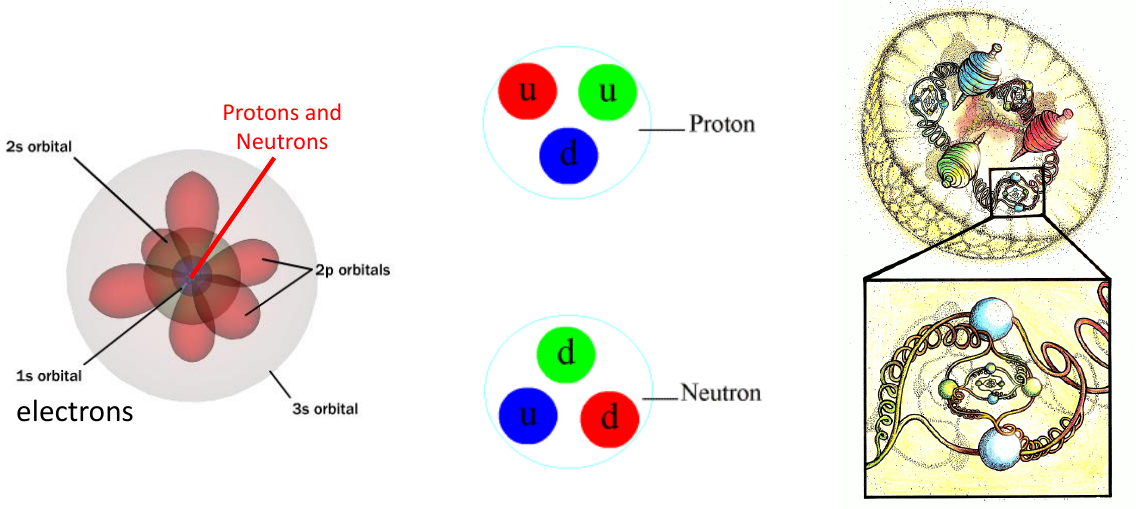
\includegraphics[width=\linewidth]{./figures/scale_of_matter.png}
	\caption{
		As we journey down further in scale, matter begins to look quite different.
		In fact, the models we use are scale dependent.
		Thomson~\ref{fig:thomsonrays}, and Rutherford~\ref{fig:rutherford} began to
		see matter as collections of atoms (left)  \cite{Freudenrich2001} (though
		not in terms of the orbital structure pictured), though it would not be
		until 20th century quantum mechanics that electron orbitals were
		discovered.  Soon, nuclei were discovered to be divisible into protons an
		neutrons  \cite{Manisearth2010} (center), which in turn were discovered to
		be composed of a sea of quarks and gluons (right). (Right image drawn by
		the talented Astrid Morreale, PhD,  \cite{Morreale2009})
	}
	\label{fig:scale_of_matter}
\end{figure}

\subsection{John Dalton}

While many had postulated the existence of atoms, the first evidence based
theory which suggested the existence of atoms was produced by John Dalton in the
early 19th century. Dalton made an important conceptual leap to relate the
existence of stoichiometric ratios in chemistry to the presence of small,
individual functional units in his experiments with chemical reactions.
Dalton's realization was only made possible due to his careful accounting of
reactants in his experiments.

It was not until Einstein's 1905 theory on Brownian Motion was experimentally
verified by Jean Perrin to place limits on the mass and size of atoms that
Dalton's atomic theory was ultimately vindicated \cite{Patterson200750}.

\subsection{J.J. Thompson}

\begin{figure}[ht]
	\centering
	\begin{subfigure}{.4\textwidth}
		\centering
		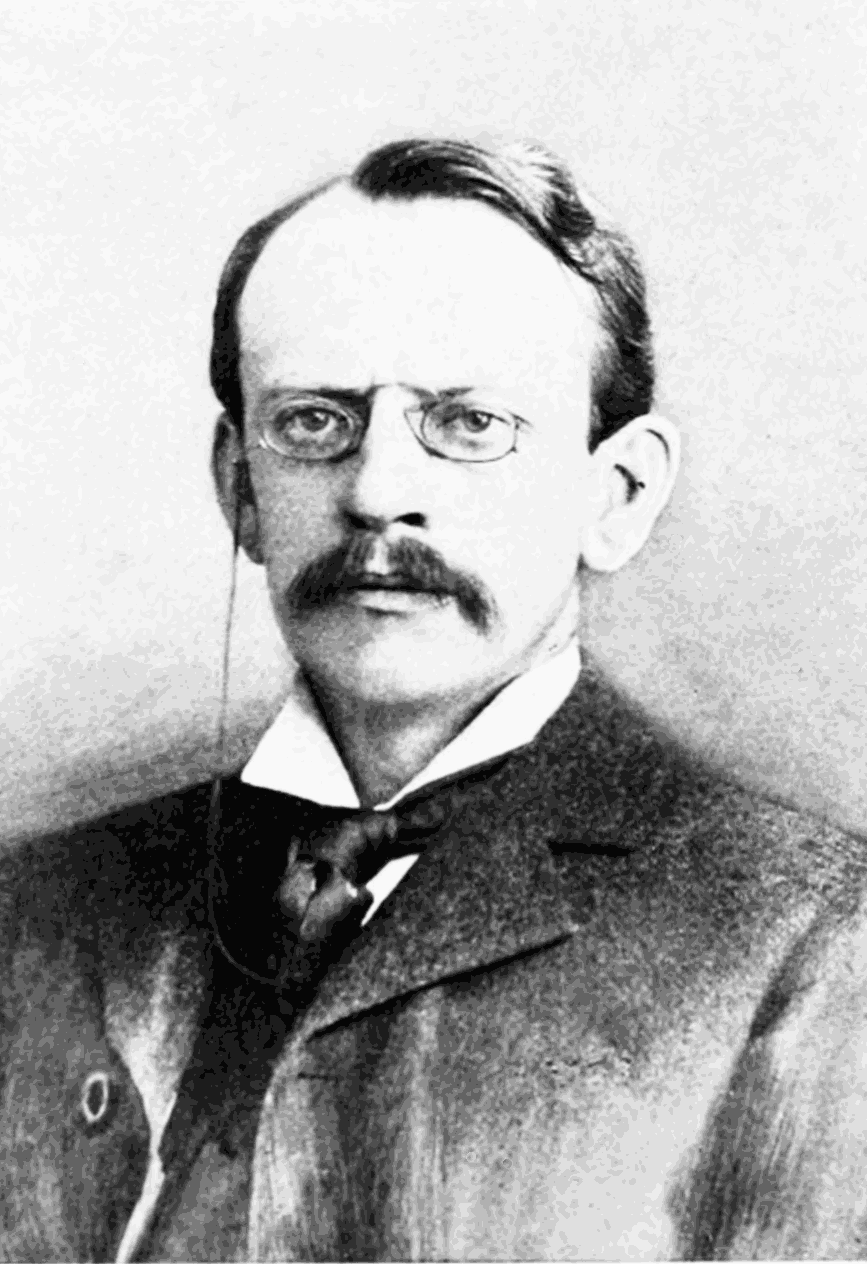
\includegraphics[width=0.4\linewidth]{./figures/jjthomson.png}
		\caption{J.J. Thomson  \cite{PopularScience1899}}
		\label{fig:thomsonportrait}
	\end{subfigure}%
	\begin{subfigure}{0.6\textwidth}
		\centering
		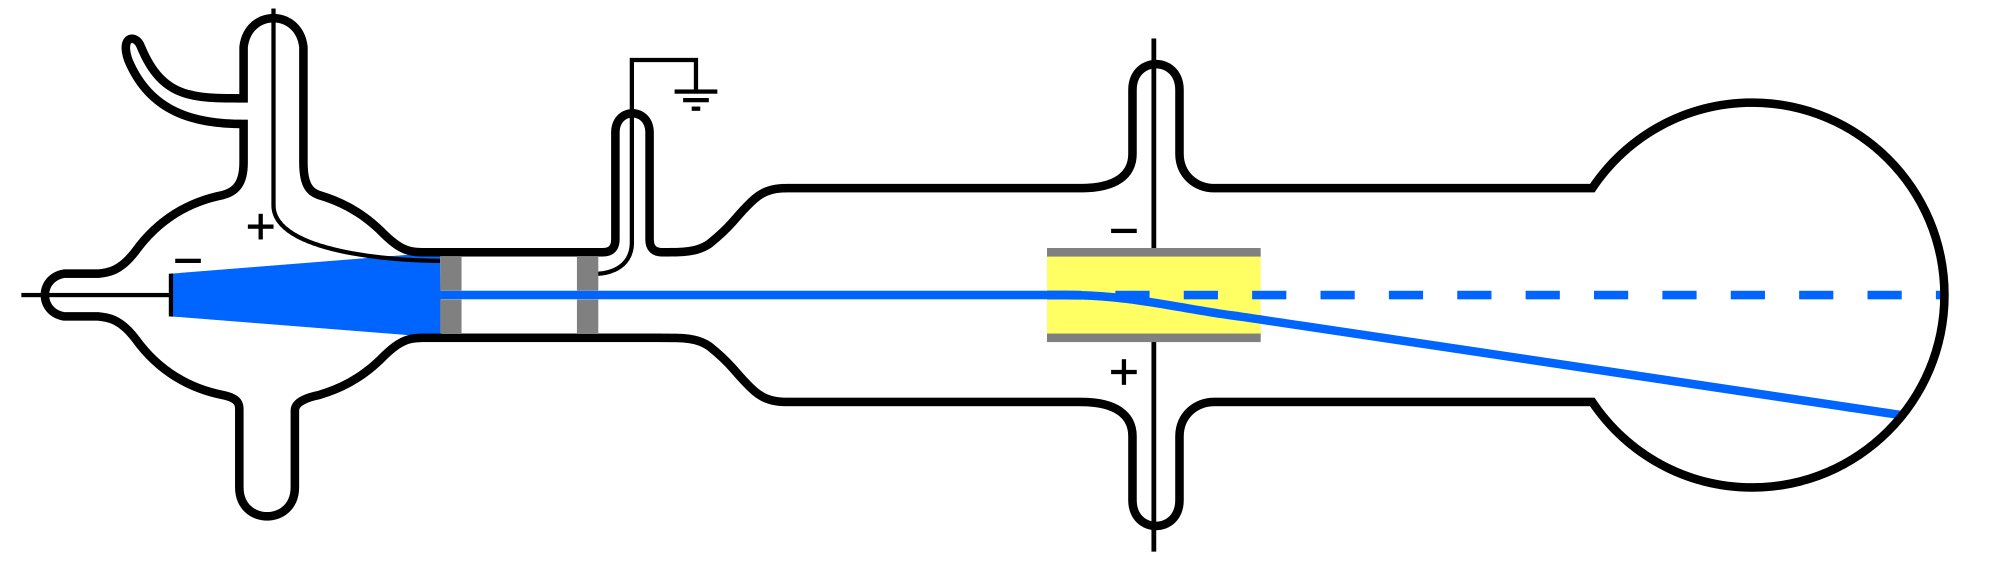
\includegraphics[width=0.4\linewidth]{./figures/cathoderaytube.png}
		\caption{Cathode Ray Tube  \cite{Kurzon2010}}
		\label{fig:thomsoncathode}
	\end{subfigure}
	\caption{ 
		Left: J.J. Thomson, who showed that cathode ray tubes were in fact producing
		the first observed subatomic particle: the electron. Right: A cartoon of
		Thomson's cathode ray tube setup. Electrons would be deflected by a magnetic
		field, sent from cathode to anode.
	}
	\label{fig:jjthomson}
\end{figure}

Thomson (Figure~\ref{fig:jjthomson}) would discover that atoms are not the
smallest, indivisible piece of matter. In his landmark experiment, he used
cathode ray scattering experiments to show that cathode rays were in fact
subatomic particles. He showed these cathode rays were identical to particles
given off by the photoelectric effect, and that these same particles were
responsible for electric current. He had discovered the electron. And, if atoms
were not the smallest piece of matter, then perhaps, atoms themselves might not
be 'indivisible' as previously thought \cite{nobelthomson2014}.

\subsection{Ernest Rutherford}

\begin{figure}[ht]
	\centering
	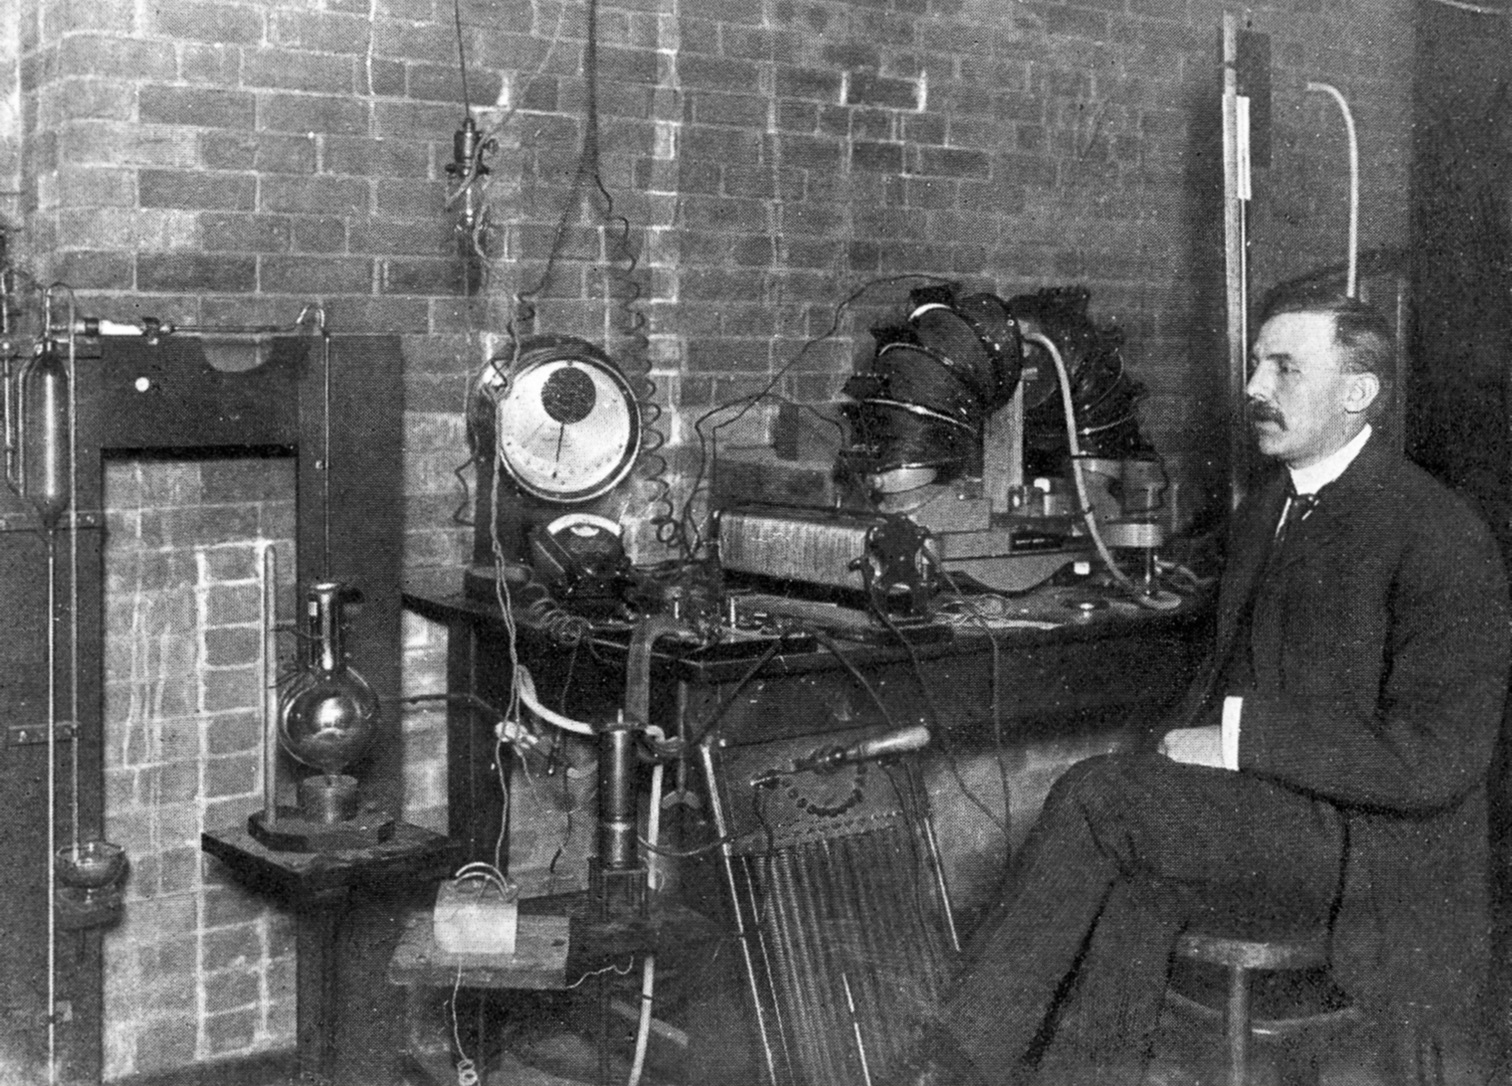
\includegraphics[width=0.6\linewidth]{./figures/ernestrutherford.jpg}
	\caption{Ernest Rutherford, in his lab.  \cite{Eve1939}}
	\label{fig:rutherford}
\end{figure}

Ernest Rutherford (Fig~\ref{fig:rutherford}) was the first to show that atoms
themselves were highly structured - and consisted of a small dense center, later
called the nucleus.

\begin{figure}[ht]
	\centering
	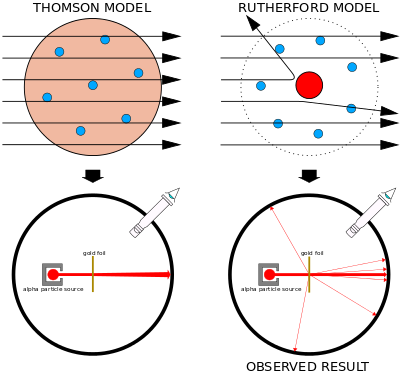
\includegraphics[width=0.6\linewidth]{./figures/geiger_marsden.png}
	\caption{
		Ernest Rutherford's historic experiment, showing (top right) that atoms were
		composed of a small dense nucleus, in contrast to Thomson's 'pudding model'
		of homogeneous charge (top left). The experiment, (bottom left and right)
		contrast the expected results (bottom left) against the observed results
		(bottom right)  \cite{Kurzon2014}.
	}
	\label{fig:geigermarsden}
\end{figure}

Rutherford's work with radioactivity was of fundamental importance, he
discovered and classified both alpha-particle radioactivity and beta-particle
radioactivity. Further studies into these types of nuclear radiation would
unlock the nucleus of atoms through the work of future scientists. Notably,
Rutherford discovered the proton.

Rutherford's proposed planetary model for the nucleus, while technically wrong,
shifted paradigms from the pudding model of  atoms, to the more familiar nucleus
+ electron cloud model which has been spectacularly modeled and verified with
the forthcoming scientists which defined the field of quantum mechanics.

Rutherford's work helped push us our of the cocoon of classical mechanics into
the weird world of the quantum mechanics - scientists would soon find that the
nucleus is not just a dense concentration of charge, but a probabilistic
structure, with rich sub nuclear structure.

\clearpage
\section{Early Quantum Theory}

During Rutherford's time, experiments were already underway which were
investigating modeling light as a wave phenomena. This was in contrast to
Newton's (unverified) corpuscular theory of light. The argument whether light
was wave-like or particle-like eventually lead to a classical field theory
describing light, and the electromagnetic interaction, yet scientists such as
Max Planck were proposing theories which required the quantization of
light~\cite{Planck1901}. Einstein would show that in his analysis of the
photoelectric effect, that light indeed was quantized into 'corpuscles'. The
nascent atomic theory of matter was also hinting at a hidden, quantized world.

\begin{figure}
	\centering
	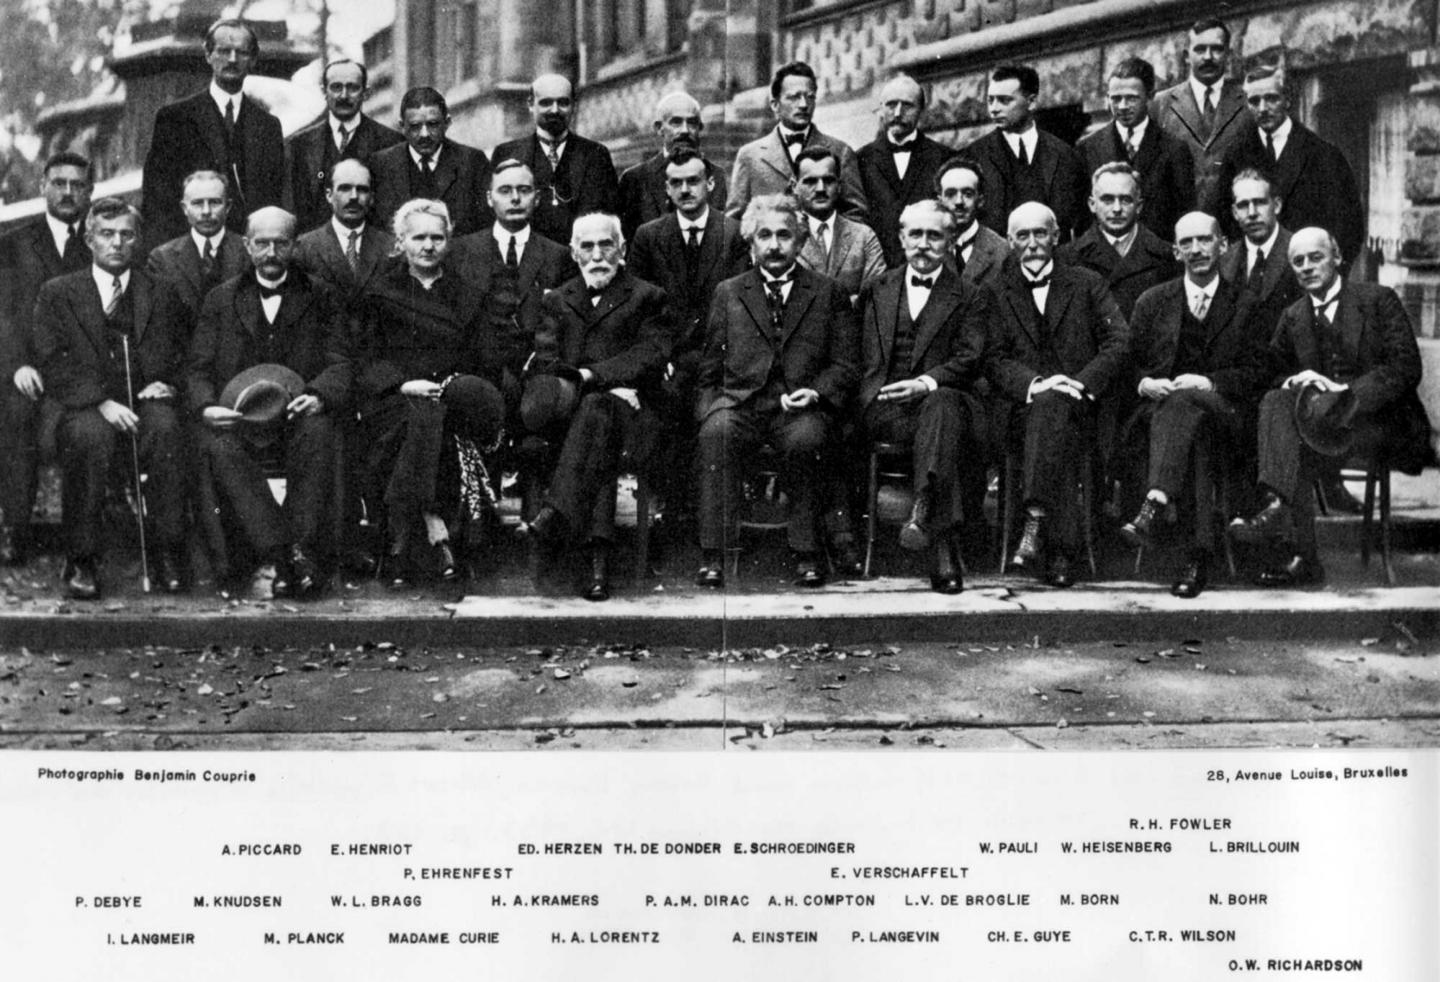
\includegraphics[width=\linewidth]{./figures/solvay.jpg}
	\caption{
		The attendees of the Solvay Conference in Brussels, 1927
		 \cite{BenjaminCroupie1927}.
	}
	\label{fig:solvay}
\end{figure}

At the Solvay Conference in Brussels, Figure~\ref{fig:solvay}, in 1927, we saw
an unprecedented gathering of some of the most important figures in modern
physics, all in one place, laying down the foundations of what would become
quantum mechanics. These scientists defined the nature and rules of quantum
mechanics - the weird model which accommodates a duality of matter - both
wave-like, and particle like. The notion that probing the structure of matter
did not yield a simple, deterministic hierarchy of structure was revolutionary,
confusing, and bizarre, and still is to this day.

It was found that not only light possesses this wave-particle duality, but also
the very particles that make up atoms as well. These models were formalized by
Dirac, Hilbert and Von-Neumann.

Though experiment tended to lead theory, regarding understanding the composition
and rules of interactions in matter, in the mid 20th century, further
refinements and additions to quantum mechanics gave birth to quantum field
theory. While early quantum models were very successful at describing static
particles trapped in static potentials - such as refining atomic theory to
include predictions of observed atomic spectra, more work was needed to
understand the relationship between electrical currents, light and magnetism.
These concepts were all related by Maxwell~\cite{Maxwell1865} in the latter half
of the 19th century, but did not make good predictions for systems in motion.

Dirac was first to create a model for describing the electron, its behavior in
electromagnetic fields, and photon emission and absorption, under fully
relativistic and quantum conditions~\cite{Dirac}. Dirac's model was so
successful, that it would become the basis for what we now call quantum
electrodynamics. Much of the mathematical formalism has been reused to describe
other field theories, which are the ultimate language which model and describe
the structure of matter - including the insides of a proton. 

\begin{figure}[ht]
	\centering
	\begin{subfigure}{.4\textwidth}
		\centering
		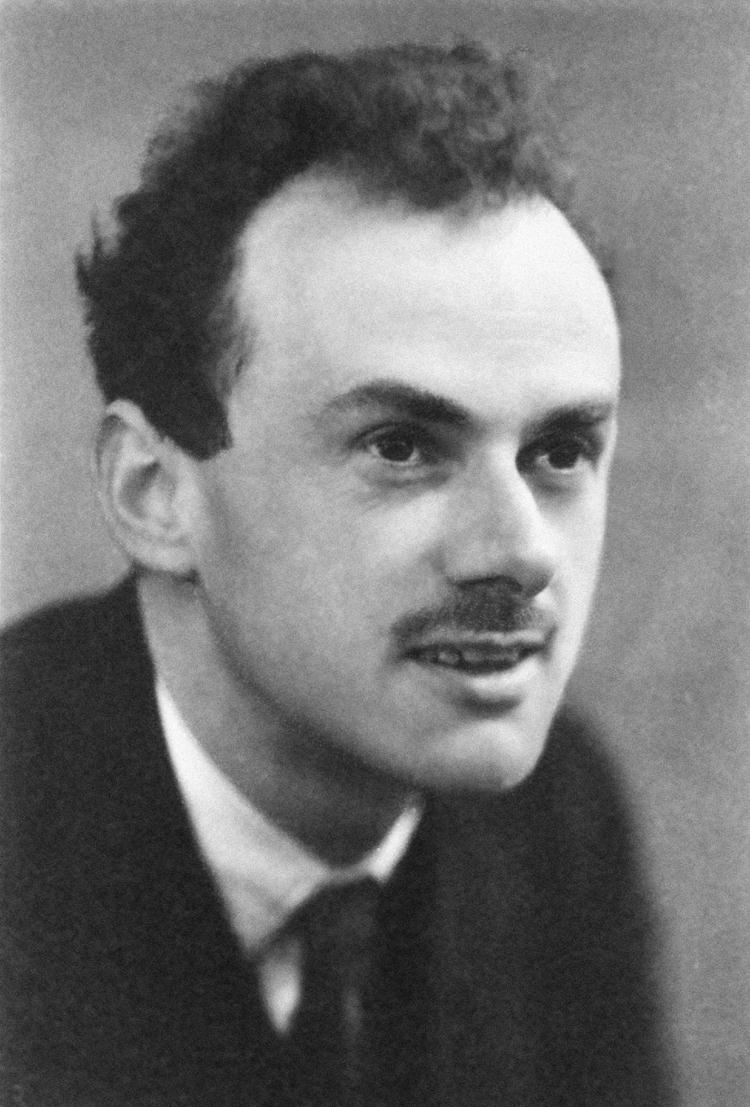
\includegraphics[width=0.4\linewidth]{./figures/pauldirac.jpg}
		\caption{Paul Dirac, 1933  \cite{NobelFoundation1933}}
		\label{fig:pauldirac}
	\end{subfigure}%
	\begin{subfigure}{0.6\textwidth}
		\centering
		\begin{equation}
			\left(\beta mc^2 + c\left(\sum_{n \mathop =1}^{3}\alpha_n p_n\right)\right) \psi (x,t) = i \hbar \frac{\partial\psi(x,t) }{\partial t}
		\end{equation}
		\caption{The Dirac Equation}
		\label{eq:diracquation}
	\end{subfigure}
	\caption{ 
		Paul Dirac, next to his original formulation of the Dirac Equation,
		describing the wave function for an electron with rest-mass $m$, in terms of
		its space-time coordinates. Dirac's equation has been expressed free of any
    defined basis.
	}
	\label{fig:thomsonrays}
\end{figure}

Dirac's work also began to incorporate relativistic effects in his wave
equations modeling the electron, as well as crucially incorporating the spin
(I.e. Dirac Spinors) of these particles, which were important for making precise
predictions for atomic spectra~\cite{Dirac}.

By this time, the proton was already known to reside in the enigmatic nucleus of
atoms, however, attempts to use Quantum Electrodynamics to describe the state of
the nucleus failed - it was clear that there was a very strong force, holding
together the protons of a nucleus tightly - far in excess of the electromagnetic
repulsion felt by the positively charged particles. There was a completely
different coupling strength between this apparent strong nuclear force, and the
better known electromagnetic coupling. Further complicating an understanding of
the nucleus is the fact that as the length scale of probing decreases, the
energies probed increase, fundamentally making the nucleus a relativistic
object. Experimental physics would once again, forge ahead, in attempting to
understand the inner workings of the nucleus, in the time-honored tradition of
performing scattering experiments.

\clearpage
\section{Early Particle Physics and The Eightfold Way}

The hydrogen atom, and its spectra was well modeled with quantum mechanics by
the end of early 20th century, however attempts to study Helium were not as
successful. However, in 1932,  when Chadwick turned a beam of
helium particles (at that time only known as $\alpha$ particles) on a sample of
Beryllium, he observed that neutral, non-ionizing, penetrating radiation was
produced  \cite{Krauss2015}. Photons were ruled out as possible
candidates, leading to the discovery of the neutron. Protons and neutrons were
hypothesized by Heisenberg to both be the same state of a new conceptual
particle, the nucleon,  \cite{Heisenberg1952}. In the same year, Anderson
discovered the positron. 

By 1934, Hideki Yukawa (Fig.~\ref{fig:hidekiyukawa}) had created an effective
field theory for interactions of 'elementary particles' (at this time, thought
to be protons and neutrons). He predicted the existence of mesons, and wrote
down an effective field theory which described how protons and neutrons bind
together in the nucleus \cite{Yukawa1935}. 

Though non-relativistic quantum mechanics was mostly complete by 1934,
scientists were already hard at work incorporating relativistic corrections to
the theory. Experiments with cosmic rays soon revealed the existence of muons
and the first observation of mesons.

\begin{figure}[ht]
	\begin{center}
		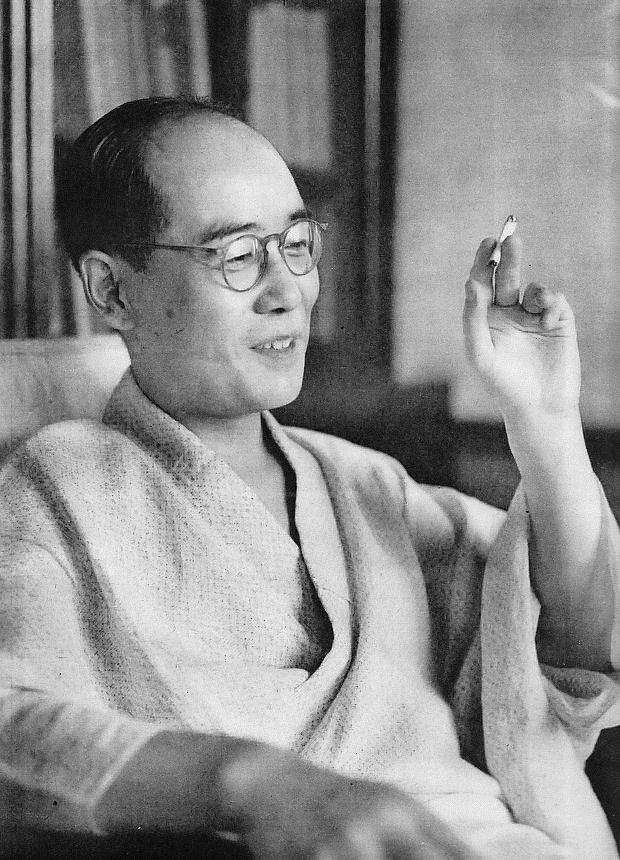
\includegraphics[width=0.5\linewidth]{./figures/hidekiyukawa.jpg}
		\caption{
			Hideki Yukawa, the first Japanese Nobel Laureate and publisher of
			influential research on the theory of mesons, and other elementary
			particles  \cite{YukawaPhoto1952}.
		}
		\label{fig:hidekiyukawa}
	\end{center}
\end{figure}

Three separate paths eventually lead to the development of particle
accelerators, which are to date, the best mechanism we possess in physics to
probe nuclear structure. These accelerators are an outgrowth
of ever more intense Rutherford-style experiments, Tandem Van-Der-Graaf
generators, resonant acceleration techniques, RF linacs, and betatron
accelerators \cite{Bryant1994}.

By the 1950's, a cornucopia of strange new particles had been discovered, both
matter and antimatter. But scientists drove forward, deeper, yearning to
discover what was fundamental. By the 50's, neutrinos had been proposed, as well
as Kaons, Pions, and Lambdas. Physicists were doing nuclear chemistry, in a
sense, attempting to work out how quickly some particles decayed, and what
decays were allowed or forbidden - science entered an age of nuclear alchemy.

"Strange" particles were discovered ($K$ and $\Lambda$), so called because in
bevatron experiments, they were produced in great quantities, but were slow to
decay, unlike the faster $\pi$ decay. Gell-Mann proposed that this strangeness
in matter was due to a new quantum number (he called it 'strangeness'). The name
stuck.
 \cite{Gell-Mann1953}, \cite{Gell-Mann1956}, \cite{Krauss2015}

The introduction of new conserved quantities, and the vast proliferation of
particles was in full swing - the subatomic world by the 1950's was confusing,
and complex. In his book "The God Particle", Leon Lederman recalled his adviser,
Enrico Fermi frustratedly remarking 'Young Man, if I could remember the names of
these particles, I would have been a botanist'. At this time, in the mid 1950's,
the number of mesons and baryons which had been discovered were at least in the
dozens, if not more.

While the use of particle accelerators were speeding us along in  our search for
the structure of matter, one particular invention truly revolutionized the
field - the bubble chamber (Figures~\ref{fig:bubble_chamber} and
~\ref{fig:bubble_tracks}.)

The bubble chamber was essentially a large vat of supercritical fluid which
could easily be caused to boil with small perturbations. This feature was
exploited, by positioning a bubble chamber in a magnetic field (to cause charged
tracks to bend) near the interaction point between a particle beam and a fixed
target. The bubble chamber itself was sometimes the target - since a popular
liquid to use was hydrogen. 

\begin{figure}[ht]
	\centering
	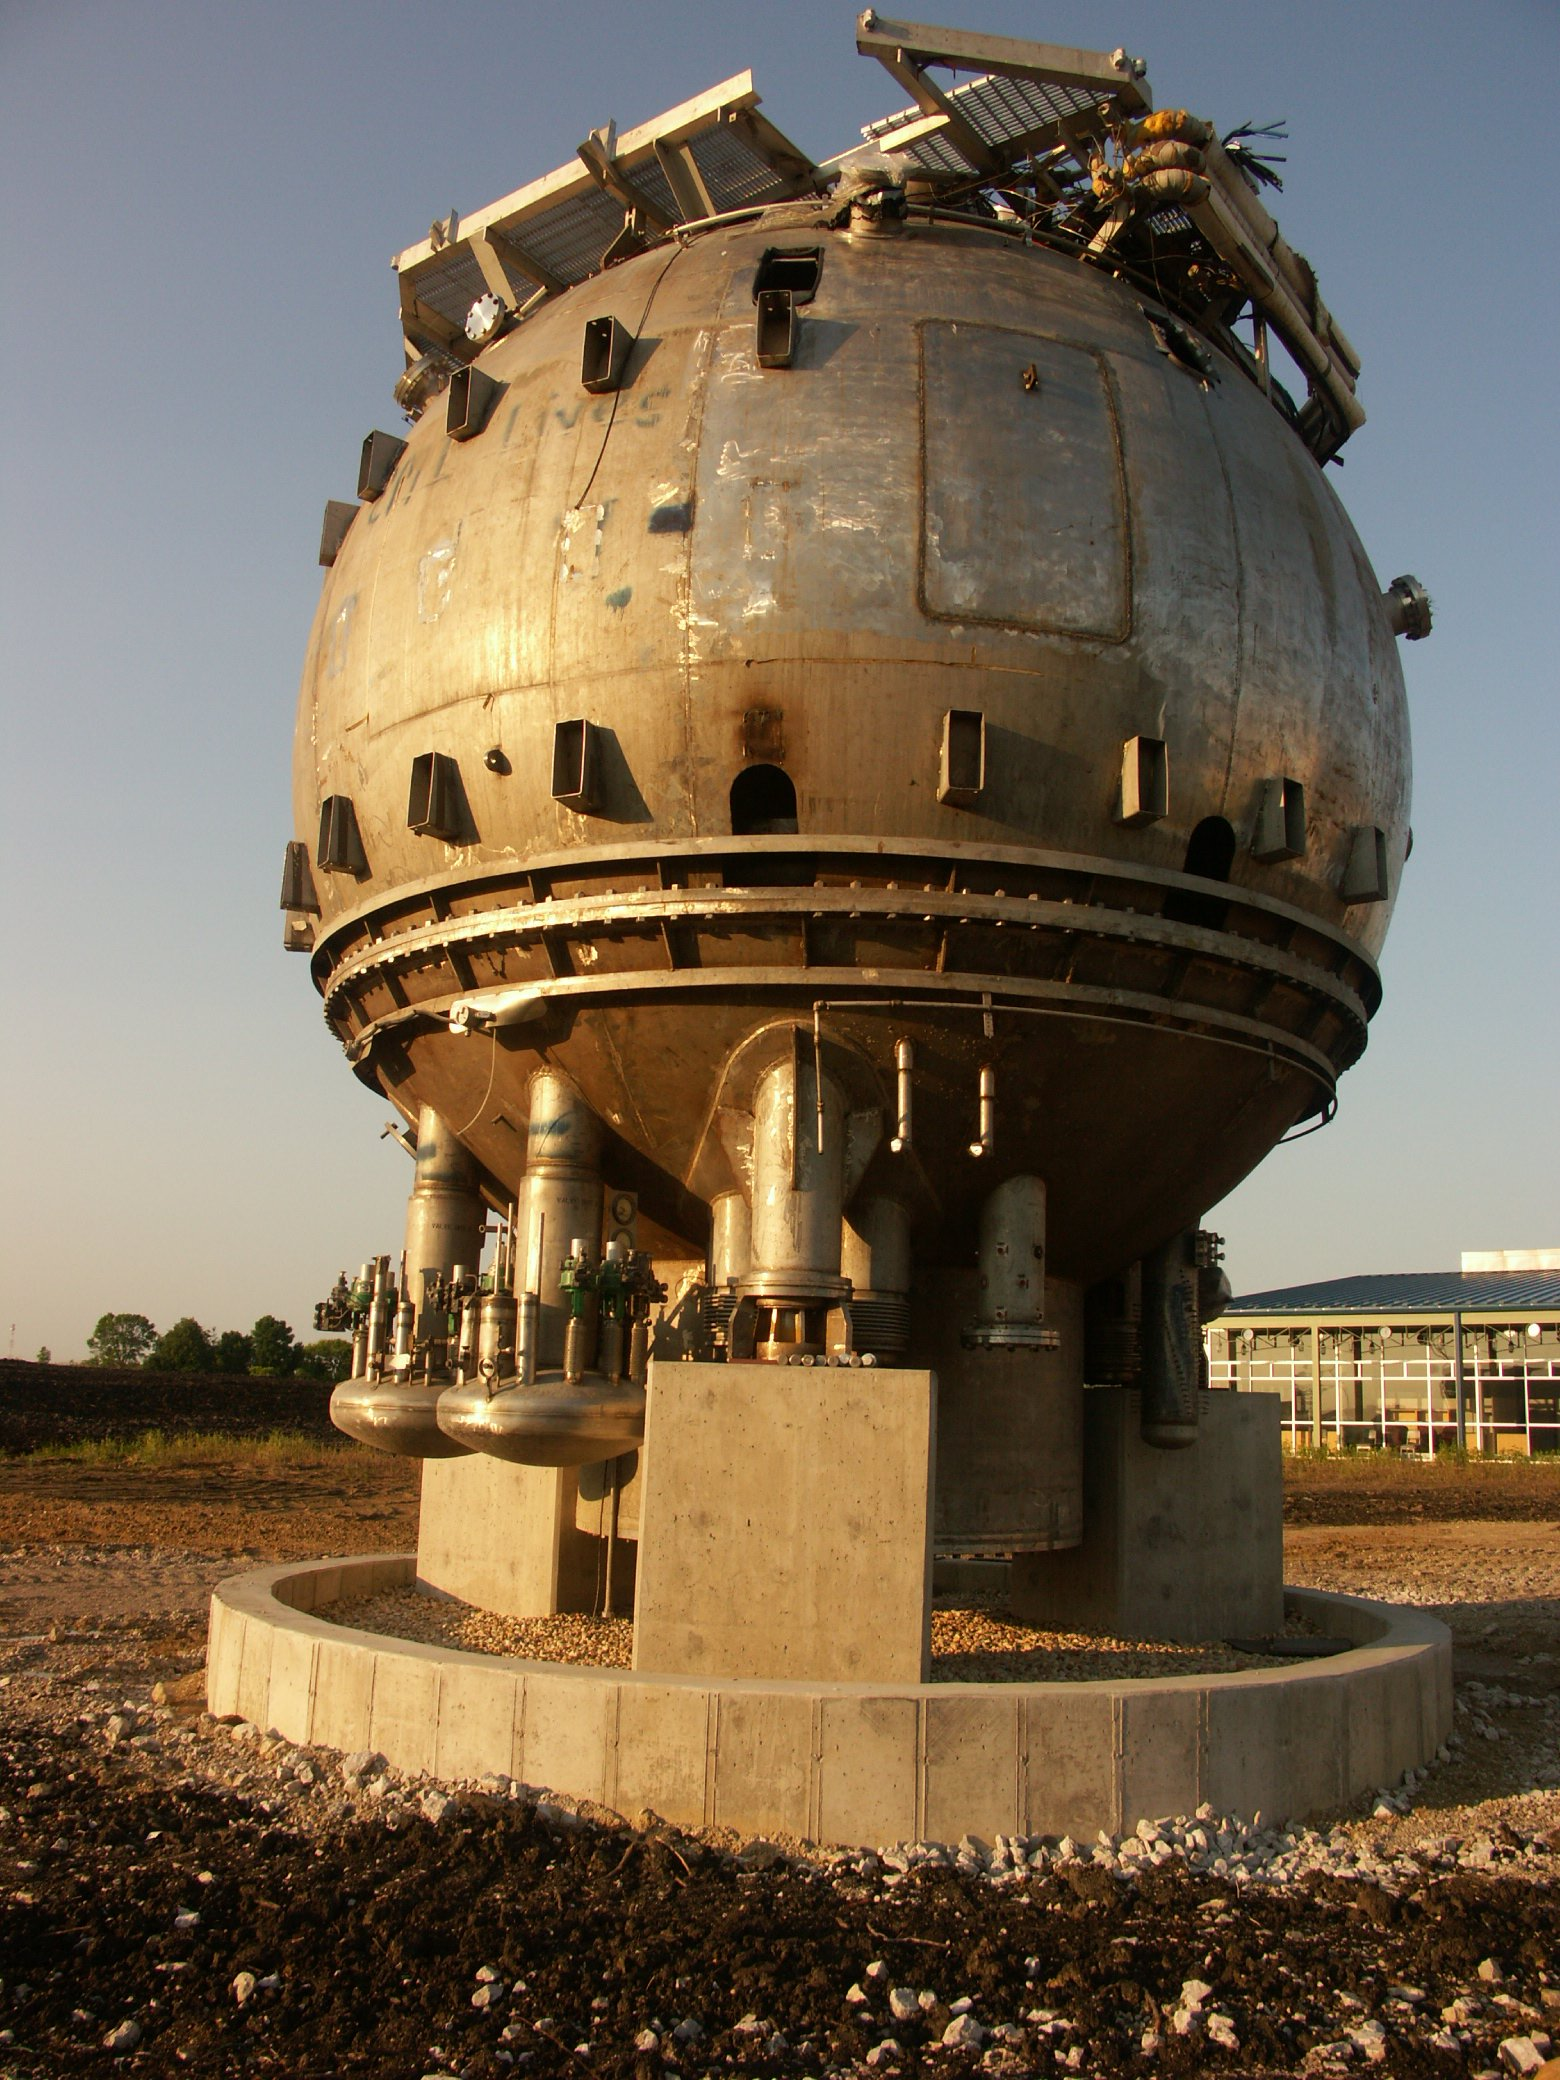
\includegraphics[width=0.5\linewidth]{./figures/bubblechamberfnal.jpg}
	\caption{An old bubble chamber, once used at Fermilab,
	 \cite{FNALBubbleChamber2005}}
	\label{fig:bubble_chamber}
\end{figure}

Invented by Donald Glaser in 1952, the bubble chamber was 'perfected' by Luis
Alvarez when he helped to develop a version which could be used with liquid
hydrogen. Hydrogen was desirable as a substance due to its extremely simple
structure, which supplied much cleaner results than other fillings, unlike the
original filler, Ether.

\begin{figure}[ht]
	\centering
	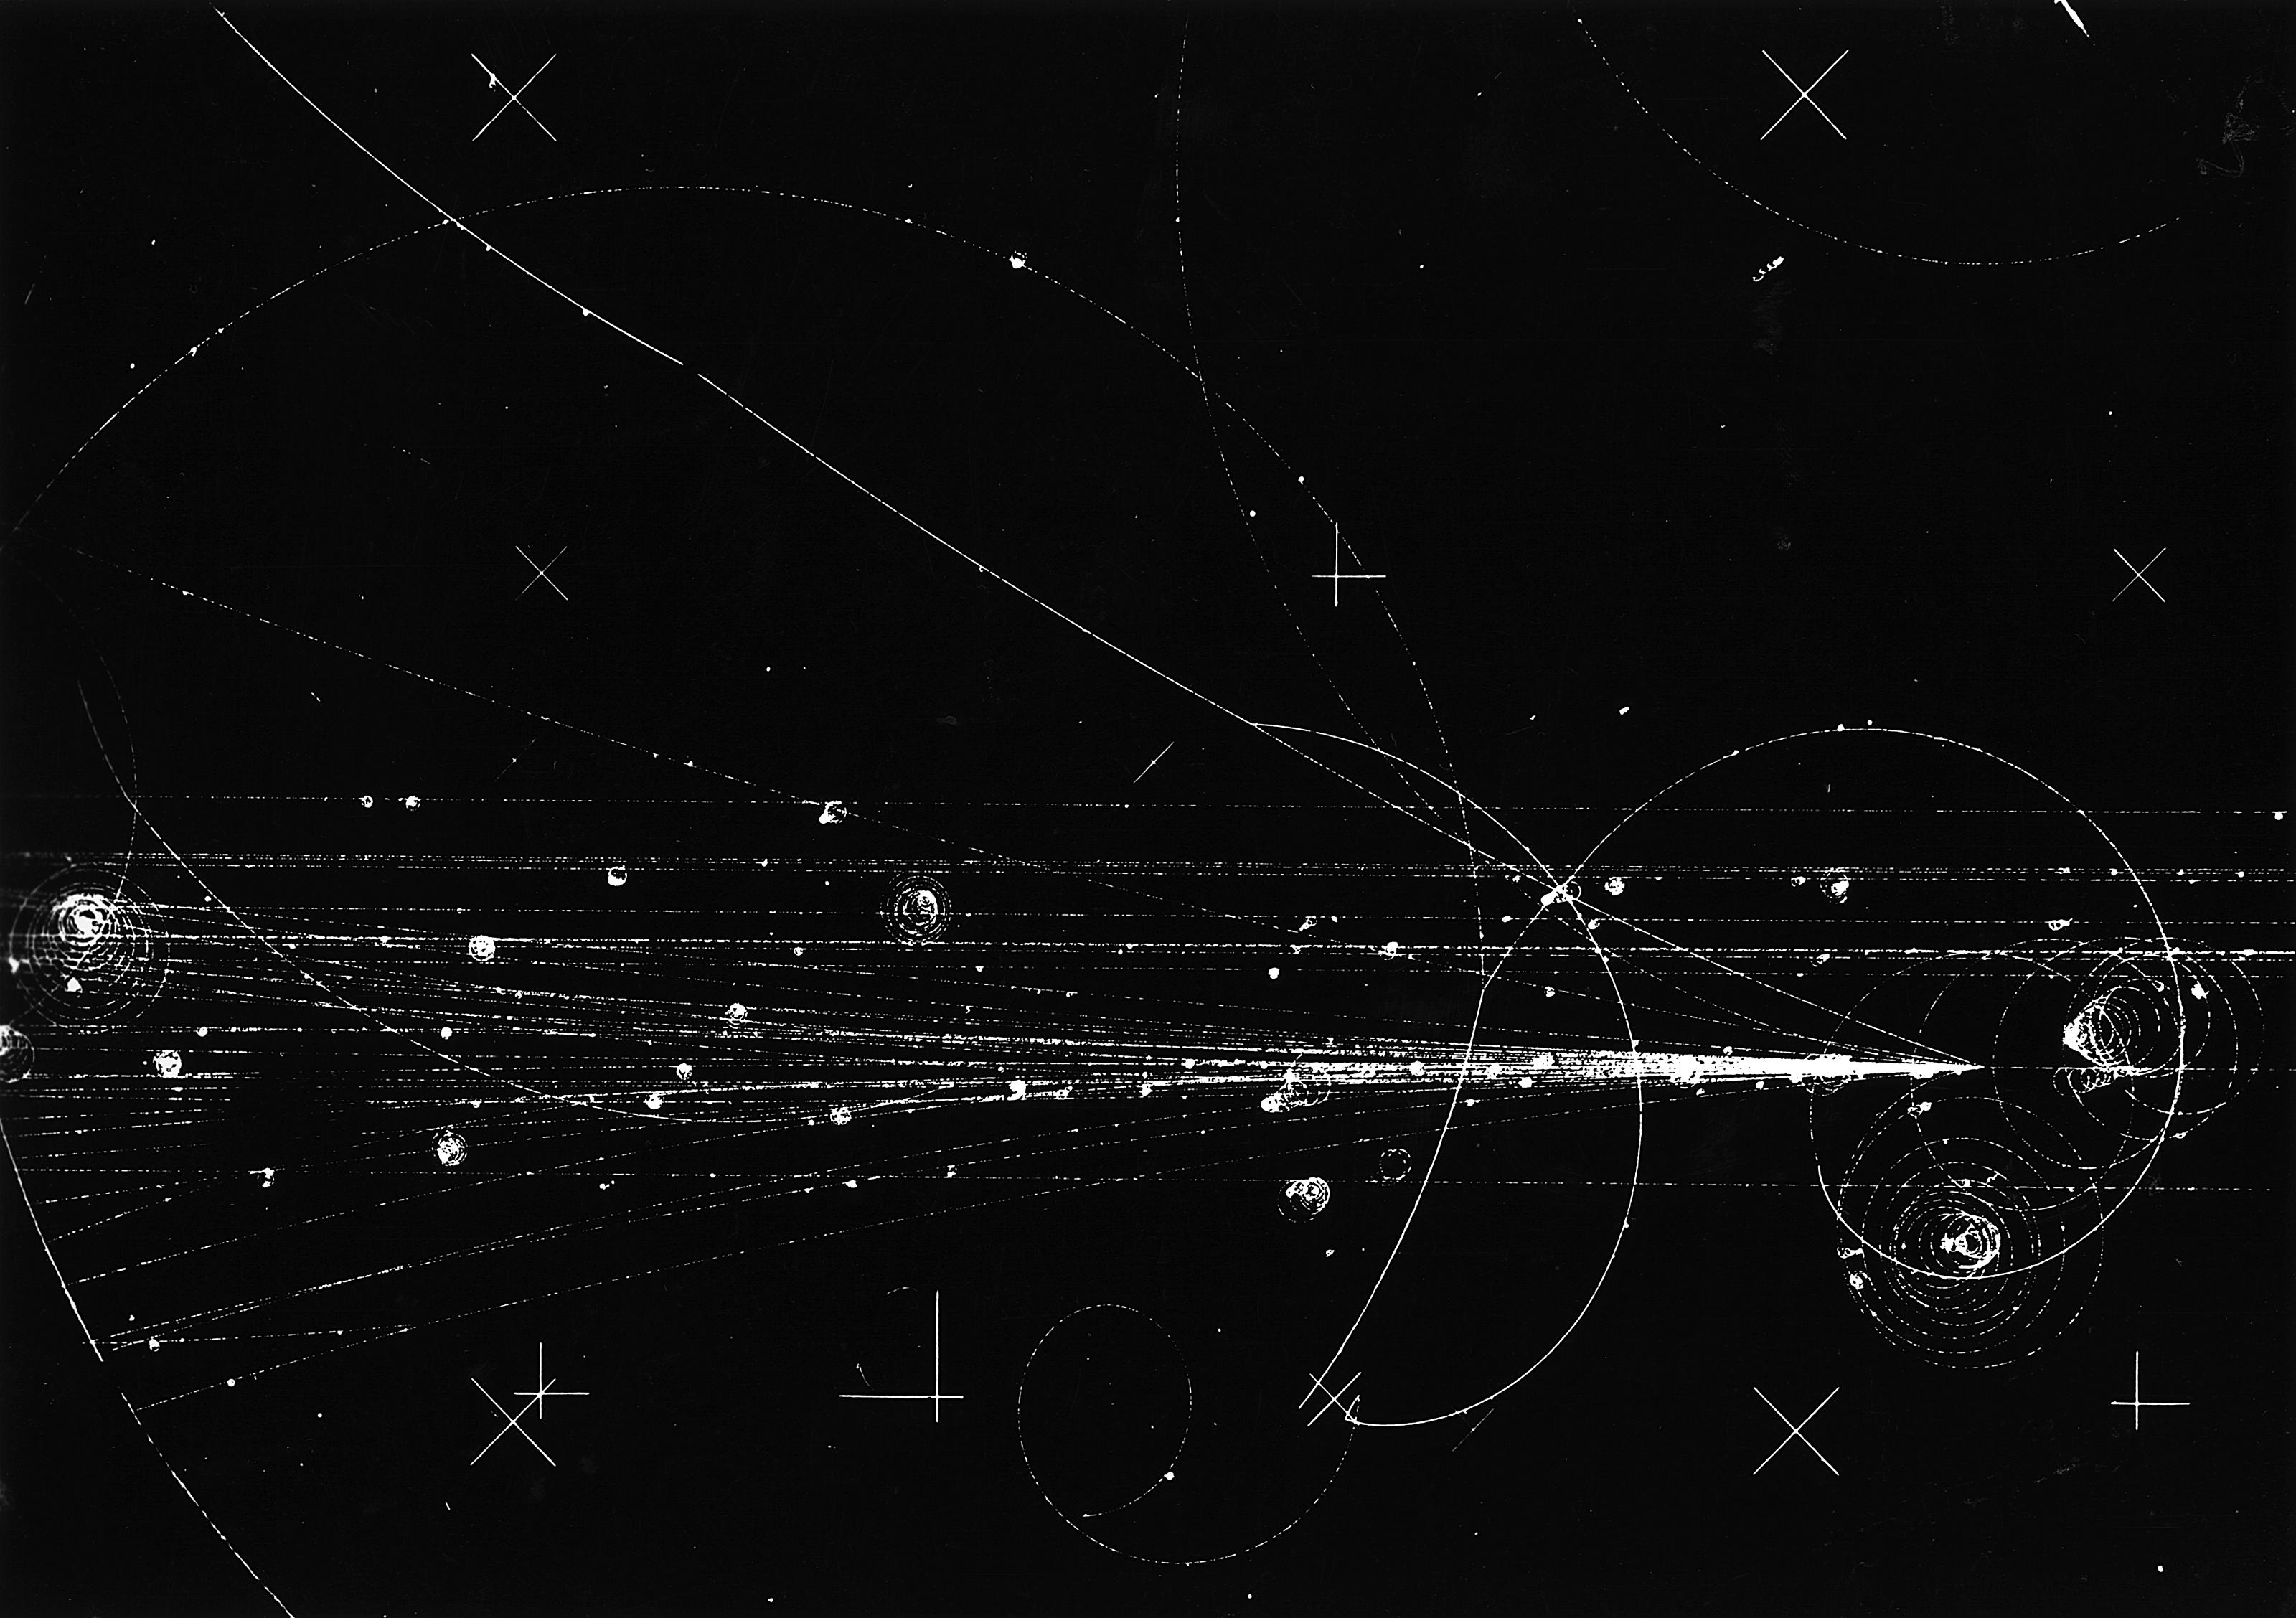
\includegraphics[width=0.5\linewidth]{./figures/bubble_chamber_tracks.jpg}
	\caption{
		An example of the photographs taken with a Bubble Chamber, in 1973.
		In this picture, we see a 300 $GeV$ proton producing particles as it travels
		through a hydrogen-filled bubble chamber at Fermilab  \cite{HD6B235}.
	}
	\label{fig:bubble_tracks}
\end{figure}

Soon after the advent of bubble chambers, physicists were able to
macroscopically image these new, exotic particles interacting with normal matter
as well as decaying - and develop novel computer techniques to analyze and
catalog the massive influx of data.

The break-through came in 1961, when Gell-Mann and Nishijima leveraged
recognized the underlying symmetry of the interactions taking place, and created
what would be known as 'the eightfold way'. This theory created a scheme for
organizing the observed baryons and mesons according to their properties in
groupings called "octets". These octets were in fact representations of the
elements of members of the $SU(3)$ group. Another way of stating this, is that
Gell-Mann had discovered the underlying structure of flavor-symmetry between the
three lightest quarks - $u$, $d$, and $s$. This work directly led to the
development of the quark model of matter, the foundation of what would become
the foundation of the standard model of particles. To date, the standard model
is the most successful theory describing particles, and their interactions.

Gell-Mann's quark model soon made important predictions which were later
verified, notably the $\Omega^{-}$, which was the ground-state particle of the
spin-$3/2$ decuplet - discovered at Brookhaven National Laboratory (the same lab
from which my research has been derived!). 

Gell-Mann formalized his quark theory of matter in 1964, however, due to the
unforeseen phenomena of color confinement, it would be several years before
evidence of quarks composing baryons and mesons was directly obtained from deep
inelastic scattering experiments.

\clearpage
\section{Quantum Chromodynamics and The Parton Model}

Deep inelastic scattering experiments, Figure~\ref{fig:disschematic} were a
natural outgrowth of Rutherford's experiment from the late 19th century. There
are a few notable differences.  Rutherford's scattering experiments can be
modeled classically, by using a classical potential as a scattering source, and
then solving as usual using an impact parameter and potential as in central
force problems. Rutherford's experiments were considered generally 'elastic'
because the target absorbed very little kinetic energy from the projectile, and
no new particles were created from the kinetic energy of the projectile-target
system.

However, in the late 20th century, scattering experiments became highly
inelastic - targets would absorb a lot of kinetic energy - sometimes so much
that targets would break apart and the kinetic energy of the system would create
particles. When referring to scattering as 'deep inelastic', the 'deep' part
refers to the process by which a scattering event occurs between a target
particle and an internal, point-like element of some complex ensemble (such as a
nucleus).

During the process of a high energy interaction between the projectile (often a
beam) and the target,  some kind of interaction occurs between the target and
the projectile, in a way that changes the state of the projectile, and generates
matter due to the high energies involved. One can observe the state of the
projectile, and account for the matter which is created, and if there are laws
which govern how the state of the projectile changes, or the kinds of matter
that can be created, then we can run the clock backwards, reconstructing the
kind of interactions that happened, to learn something about nuclear structure
(or even partonic structure). In this way, one can also identify conserved
quantities, which in turn suggest physical symmetries, which in turn help to
build models.

One can think of interaction of a beam and target in terms of a probability of
interaction - and this formalism will be discussed further in chapters related
to the Vernier Analysis I worked on. Succinctly, however, one can mathematically
'separate' part of this interaction probability into a quantity called a
'cross-section', often denoted as $\sigma$ for a total cross section, or
$d\sigma$ for a differential cross section, or even ${d\sigma}\over{d\Omega}$ to
refer to a differential cross section scattered into a solid angle. The $\sigma$
of any scattering experiment can be represented many different ways.

From a theoretical standpoint, we can represent protons (and other baryons) by
selecting the relevant internal degrees of freedom we may want to study, and
then devising some rules for the internal structure. We may be interested in the
momentum fraction carried by some distribution of partons, or how the relative
populations of partons within a certain kinematic regime changes with
distance/energy scale. For all of these cases, we use parton distribution
functions, or structure functions. Concretely, these functions depend on:


A subcategory of deep inelastic scattering is 'Semi-Inclusive Deep-Inelastic
Scattering'. This refers to a case where a beam (say a lepton, such as an
electron) interacts inelastically with a point-like internal structure of a
target particle, and a hadron is produced (such as a $\pi^+$), which is then
detected. Semi-Inclusive Deep-Inelastic scattering is then the process by which
the scattered lepton and a specific hadron are measured in the final state of
the interaction (but other particles that might be produced are neglected or
ignored).

I said the word parton, which I have been carefully avoiding, but now the cat's
out of the bag. Nuclei, as we will learn, are not elementary particles, but
instead, are built up from what we assume are fundamental, elementary particles.
Deep inelastic scattering experiments slowly revealed that nuclei (individual
protons and neutrons) were not elementary particles, but instead, composite
particles. It is natural to assume then, that the properties of protons and
neutrons are not fundamental either. And in fact, the vast zoo of particles that
were discovered in early inelastic scattering experiments, such as $\pi$ or $K$
or $\Lambda$ (discussed briefly earlier) were not fundamental either.

In Michael Riordan's excellent 1992 summary of the discovery of quarks, Riordan
lays out a very succinct and thorough history of the late 20th century
experimental and theoretical works which built on Rutherford and Gell-Man's
work. Riordan states that surprising 'results came from a
series of electron scattering experiments...from 1967 through 1973' at MIT and
SLAC, which comprised the first set of evidence produced in favor of the
partonic model. As described earlier, Gell-Mann created a three-quark model to
produce predictions consistent with these observations \cite{Riordan1992}.

\begin{figure}[ht]
	\centering
	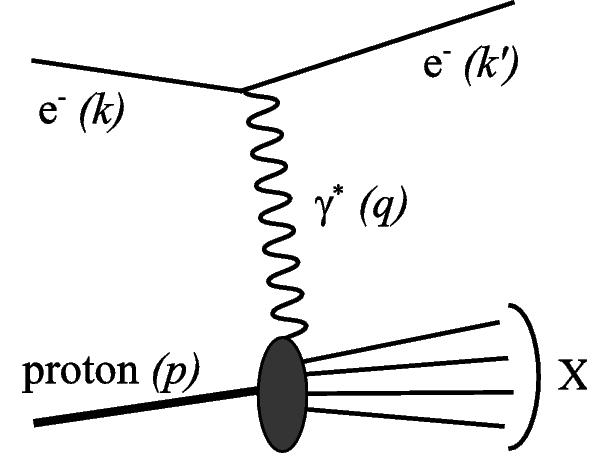
\includegraphics[width=0.6\linewidth]{./figures/deep_inelastic_basic.png}
	\caption{
    A schematic~\cite{Ddn2_2008} of deep inelastic scattering, where the
    incoming electron inelastically scatters off the proton, producing results
    $X$, via virtual photon exchange, $\gamma^*$. The diagram is split into a
    perturbative portion (the electron) and a non-perturbative portion.
    Mathematically, we describe the interaction with kinematic variables
    summarized in Equations~\ref{eq:P}-\ref{eq:x}
  }
	\label{fig:disschematic}
\end{figure}

By the 1970's, collaborations between Bjorken, Feynman, and others had produced a
coherent partonic model which contained quarks, and force mediating gluons.
Additionally, the concept of Structure functions had been developed. Modified
from Rutherford's original scattering formula, this new formula to describe the
cross section of deep inelastic scattering incorporated structure functions,
which separated out the momentum exchange between target and projectile (via a
virtual photon), and isolated this from $W_1$ and $W_2$, structure functions
which were experimentally measured quantities representing the electron-proton
interaction (the 'physics-y' part of the interaction).

This period of time, from 1970 - 1990 was truly the golden age of Deep Inelastic
Scattering Experiments - the biggest laboratories running experiments were (and
some are still running) The European Organization for Nuclear Research (CERN),
The Stanford Linear Accelerator Center (SLAC), and The German Electron
Synchrotron (DESY). Thousands of papers were published - some groundbreaking,
such as the CERN's European Muon Collaboration experiment which showed a
measurement of the spin asymmetry and determination of the proton structure
function $g_1$ in muon-proton deep inelastic scattering  \cite{Ashman1988}. 

The formalism of scattering theory continued to evolve during the booming period
of particle physics from 1960 to present day. Though the mechanics of scattering
experiments have remained essentially unchanged, vast improvements in technology
in detectors, data collection and reconstruction, and beam production have
evolved from Geiger and Marsden's humble beginnings to create scientific
measurements of particles and their properties with exquisite and unprecedented
precision. The kind of precision I'm talking about is exemplified in Brookhaven
National Laboratory's E821 Muon ($g$-$2$) experiment - which measured the
anomalous magnetic moment, $g$-$2$, of the muon to a precision of 7 parts in ten
million  \cite{Bennett}.

The advent of structure functions hailed an era of non-point-like baryonic
matter. The mathematics of scattering formalism had to change to accommodate the
underlying physical distribution of partonic matter in baryons. Deep Inelastic
Scattering continued to probe various portions of these structure functions, and
the structure of the standard model began to come into focus, distilled into the
relatively simple mathematical structure of group theory. Concretely, the
standard model is a gauge theory, which contains the internal symmetries of
$SU_{c}(3) \times SU_{L}(2) \times U_{Y}(1)$, Figure~\ref{fig:standardmodel}.
The Standard Model is said by some to be "complete" with the discovery of the
Higgs Boson, yet with emergent phenomena such as proton spin, it does not
provide a straightforward prediction. The model still has not included
gravitation and relativistic effects fully - and probably isn't entirely
correct.

\begin{figure}[ht]
	\centering
	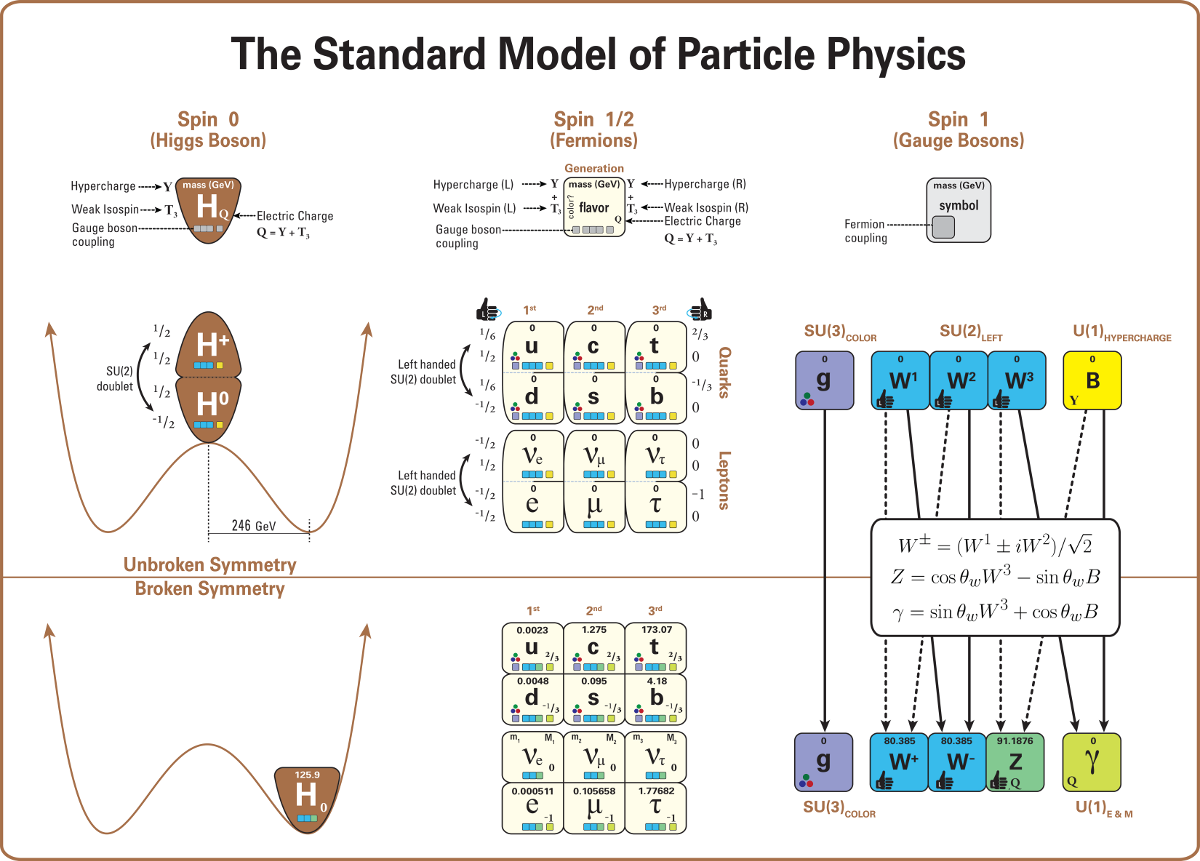
\includegraphics[width=\linewidth]{./figures/standard_model_complete_lowres.png}
	\caption{
		"This diagram displays the structure of the standard model (in a way that
		displays the key relationships and patterns more completely, and less
		misleadingly, than in the more familiar image based on a 4x4 square of
		particles). In particular, this diagram depicts all of the particles in the
		standard model (including their letter names, masses, spins, handedness,
		charges, and interactions with the gauge bosons -- i.e. with the strong and
		electroweak forces). It also depicts the role of the Higgs boson, and the
		structure of electroweak symmetry breaking, indicating how the Higgs vacuum
		expectation value breaks electroweak symmetry, and how the properties of the
		remaining particles change as a consequence."\cite{Boyle2014}.
	}
	\label{fig:standardmodel}
\end{figure}


\clearpage
\section{The Era of Deep Inelastic Scattering}

Here, I hope to highlight the last 40 years or so of physics produced by deep
inelastic scattering experiments. We are now truly in an era of 'Big Science',
where the boundaries of science are pushed by huge collaborations of men and
women working together. 

Since the era of deep-inelastic scattering brings us essentially up to speed
with the physics needed to address the rest of this thesis, I will be rather
broad in this final section of this chapter, sparing the explicit details for
the next chapter.

This era of deep-inelastic scattering has unearthed some of the most surprising
and monumental discoveries in physics - all the way from the recent discovery of
the particle mediating the field that imbues all fundamental particles with
mass, to the discovery that protons and neutrons are not fundamental particles
at all, but are instead, highly relativistic balls of gluons.

The models trying to predict and describe the behavior of the proton and
neutron, as well as the physics that creates a nuclear bound state have been in
development since the late 1950's. By the late 1970's, we begin to approach a
description of nuclear partons that closely resemble what we see in present day.

The early days of deep inelastic scattering led to the discovery of many of the
fundamental particles we know and love today, in the standard model. The
precise way these particles forms baryonic matter was not initially well
understood, though with the introduction of structure functions and parton
distribution functions, we began to make progress.


SLAC's E\#\#\# (E80-E155) were some of the first experiments to probe the proton
spin structure, operating from 1978-1999. SLAC pioneered the usage of spin
asymmetries as a means of ruling out models for various parameterizations of
quark structure functions, as well as provided important data constraining
nuclear structure functions. SLAC's experiments focused on understanding the
spin structure of the quarks (but not gluons) within protons.

The European Muon Collaboration at CERN was one of the first major international
efforts to get underway studying the underlying structure of protons and
neutrons with deep inelastic scattering. The collaboration produced scientific
results from 1979 to 1997. The EMC's major contribution to our understanding of
nuclear structure was to amass evidence which supported the parton model of
protons and neutrons, as well as discovered the self-named 'EMC effect', which
showed that the volume 'occupied' by quarks scales with heavier
nuclei~\cite{Aubert1983}. The EMC also elucidated the effects of quark
fragmentation and hadron production, DIS in the nuclear medium, and produced
some of the first measurements of the spin structure of the proton. Most
famously, the EMC originally discovered the 'proton spin crisis' in its first
measurement of the proton spin structure function, $g1$ where it found the spin
carried by the proton's 'valence quarks' to be less than 1/2~\cite{Ashman1988}. 

CERN also produced another collaboration which contributed to our understanding
of nuclear structure - the Spin Muon Collaboration. The SMC was active from 1993
to 1998, used polarized beams of muons shone onto a polarized target (ammonia
and later p-butanol) to measure a virtual photon production asymmetry $A_1$ in
order to measure information about the structure function, $g_1$ (discussed in
detail in the following chapter). $g_1$ gives access to the quark polarization
of protons. Spin structure physics has been explored at the COMPASS experiment
since 2005. CERN's work to understand the spin structure of the proton probed
the contributions of both the quark, and gluons. 

In Germany, DESY is the premier accelerator science laboratory, and has been
operating continuously since 1964. DESY's primary experiments in deep inelastic
scattering with regards to nucleon structure have been underway since 1992. DESY
operates several important deep inelastic scattering experiments including ZEUS,
HERA (H1 and H2) and HERMES. The scientific goals of DESY are much broader,
since it represents Germany's premier accelerator physics scientific effort,
including fields such as condensed matter physics and astrophysics. However, the
portion of DESY's research program devoted to spin structure seeks to understand
both the quark and gluon contributions to proton spin.

Jefferson Laboratory (JLab) is an electron accelerator complex in Virginia
specializing in the cutting edge of fixed target electron deep inelastic
scattering experiments. Experiments in Hall A, B and C are all involved with
studying both quark and gluon contributions to proton spin.

Of course, an important unmentioned player in the modern era is the Relativistic
Heavy Ion Collider, and the experiment PHENIX. The cumulative results of these
experiments and how they inform this thesis research with regards to our probing
and modeling of the structure of protons  are presented in the following
chapter.
